\section{Introduction}
We are interested in designing autonomous systems that can perform
complex mobile manipulation tasks over long time horizons (e.g.,
setting a dinner table, doing laundry). We approach this problem in
the framework of combined \emph{task and motion planning} ({\sc tamp}).

In {\sc tamp}, an agent is
given a symbolic, logical characterization of actions (e.g., move,
grasp, putdown), along with a geometric encoding of the
environment.  Efficient integration of high-level, symbolic task planning
and low-level, geometric motion planning is
difficult; recent research has proposed several methods for
it~\cite{srivastava2014combined, deardenplanningtamp, kaelbling2011hierarchical,
  lagriffoul2014orientation, GarrettWAFR14, dornhege2012semantic}.
We adopt the principles of abstraction in the {\sc tamp} system developed by
Srivastava et al.~\cite{srivastava2014combined} (henceforth referred
to as {\sc sfrcra-14}) to factor the reasoning and search problems into
interacting logic-based and geometric components.

\begin{figure}[t]
  \centering
    \noindent
    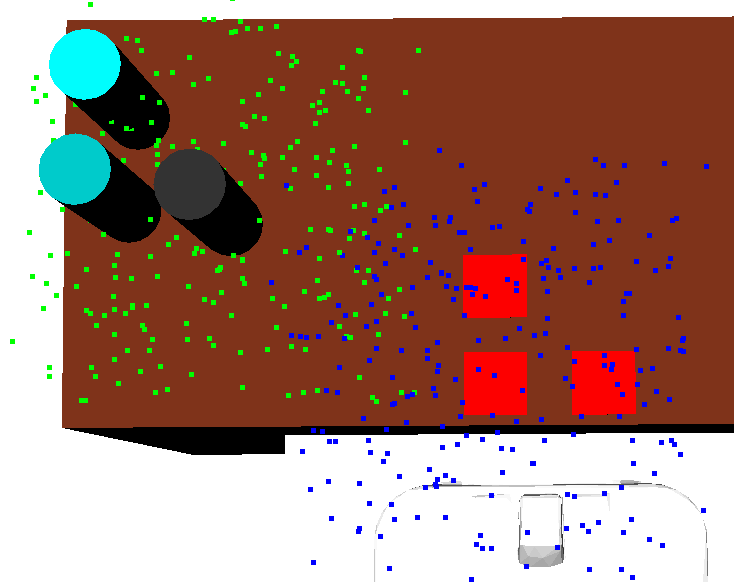
\includegraphics[scale=0.112]{images/learns.png}
    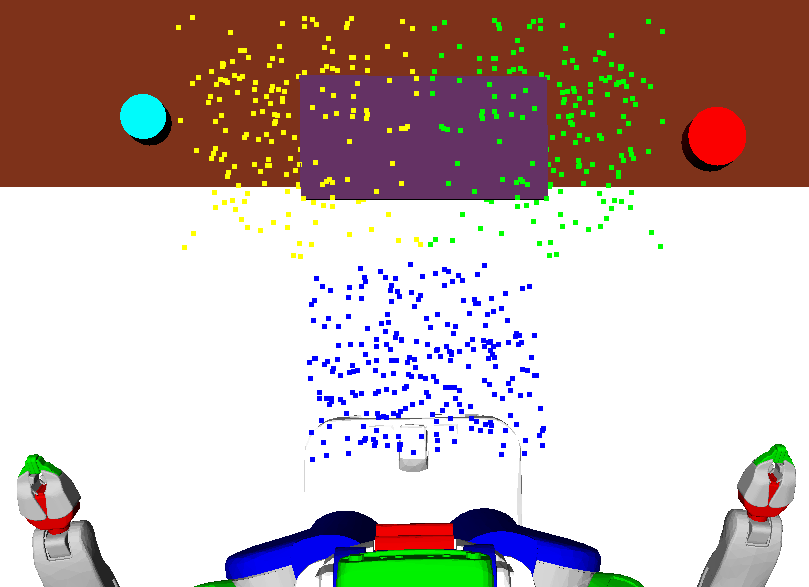
\includegraphics[scale=0.13]{images/dinner_tray_initial.png}
    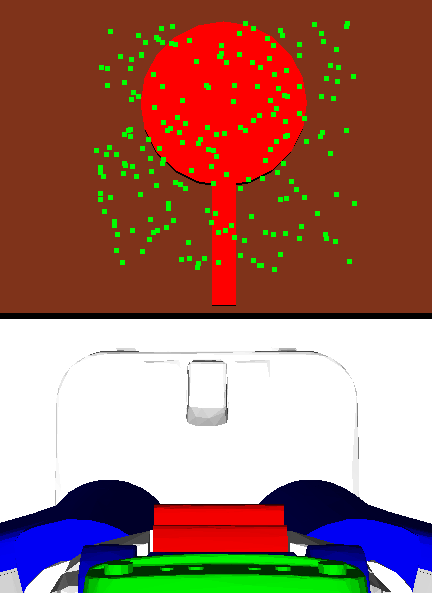
\includegraphics[scale=0.13]{images/frying_initial.png}\vspace{1em}
    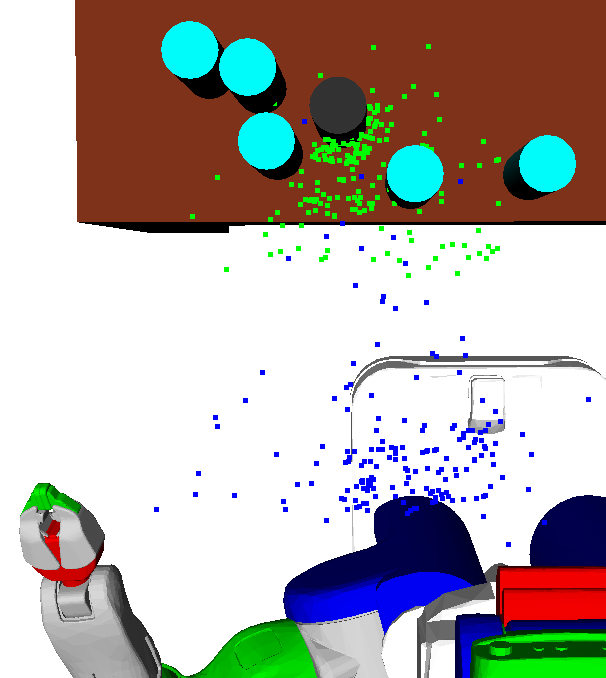
\includegraphics[scale=0.112]{images/learn12.png}
    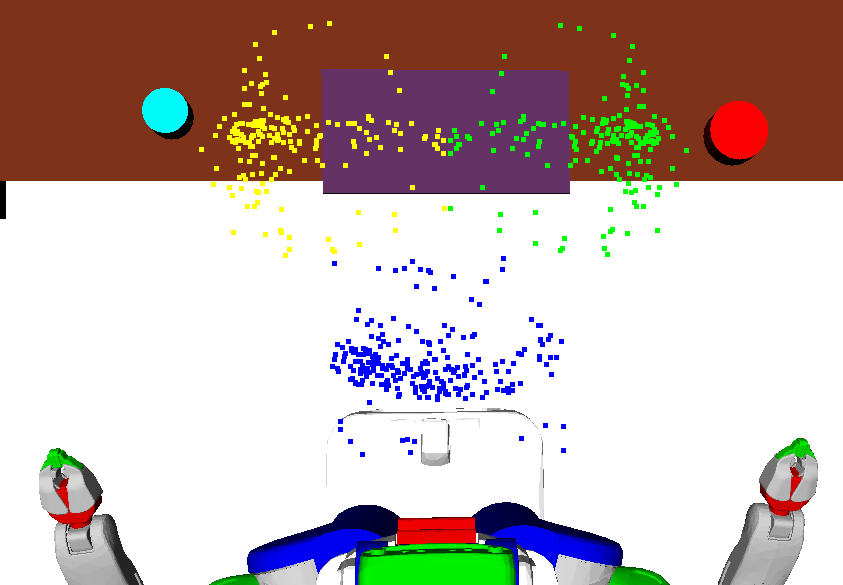
\includegraphics[scale=0.13]{images/dinner_tray_final.png}
    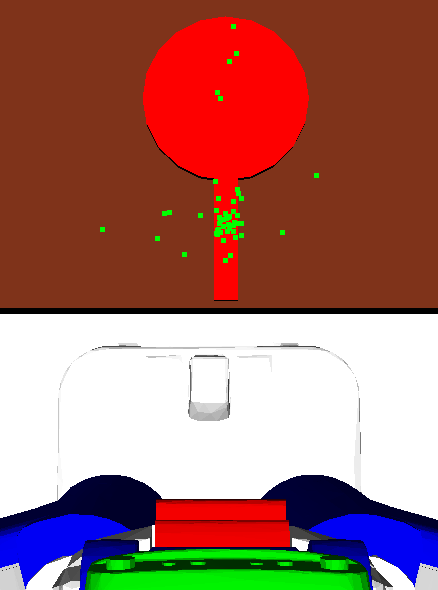
\includegraphics[scale=0.13]{images/frying_final.png}
  \caption{\small{We use reinforcement learning to train sampling distributions for
      continuous motion planning parameters in long-horizon tasks. The top images show
      initial, uniform distributions. The bottom images show learned base position (blue) and
      grasping (green, yellow) distributions for picking up various objects in our simulated domains:
      a can (left), a tray (middle), and a frying pan (right).
      The green and yellow points refer to the positions of the tool center points;
      the end effectors are oriented to point toward the object being grasped. The can and
      frying pan are picked up using only one gripper.}}
  \label{fig:cover}
\end{figure}

In this work, we develop a complete algorithm for {\sc tamp} and propose learning
methods to perform joint guided search in the space of
high-level, symbolic plans and their low-level
\emph{refinements}: instantiations of continuous values for
symbolic references in the plan. For example, in a pick-place domain, a high-level plan
consists of a sequence of move, grasp, and putdown actions, while its refinement is a sequence of
collision-free trajectories that implement the plan. We refer to the search for a valid
refinement as \emph{plan refinement}.

{\sc sfrcra-14} uses error information propagated from the geometric planner
to update the symbolic state and generate a new high-level plan.
For example, if motion planning discovers obstruction information in a pick-place domain, the
new plan may involve moving the obstruction out of the way.
In our work, we think of these errors as defining a \emph{plan refinement graph} whose nodes are high-level plans
and edges are error fluents. We develop a complete algorithm that interleaves
search over this graph with plan refinement.

We present machine learning techniques that guide
search over both the low-level plan refinement and high-level plan refinement graph.
Both search spaces are very large, so we need heuristics to make search efficient.
At the low level, this amounts to
learning to propose continuous values for symbolic references that are likely to result in
collision-free trajectories. Many {\sc tamp} systems rely on hand-coded heuristics to
account for these continuous parameter settings. This often requires
domain-specific insight from the user to reduce the search space.
We apply reinforcement learning ({\sc rl}) to learn domain-specific distributions
over these values in a domain-independent fashion.
At the high level, training heuristics amounts to learning
how difficult it is to refine a given plan. Directly applying reinforcement learning
for this is challenging because taking actions in this space requires attempting to
refine a plan, which can be time-consuming. Also, for complex tasks, there are often many candidate high-level plans that
achieve the goal. Instead, we use inverse reinforcement learning
based on expert demonstrations to train heuristics at this level.

Our low-level learning approach draws inspiration
from Zhang and Dietterich~\cite{JobShopSched}, who applied {\sc rl} to job
shop scheduling. In their formulation, states correspond to schedules
and actions propose changes to the schedule. In our setting, states
correspond to (potentially infeasible) refinements and actions propose
new values for symbolic references.

The contributions of our work are as follows: 1)
we present a complete algorithm for {\sc tamp}; 2) we present a randomized
local search algorithm for plan refinement that is easily formulated
as an {\sc mdp}; 3) we apply {\sc rl} to learn
a policy for this {\sc mdp}; 4) we learn from expert demonstrations to
efficiently search the space of high-level plans,
given options that address different infeasibilities; and 5)
we run experiments to evaluate the performance of our system in a
variety of simulated domains. Our results demonstrate
significantly improved performance over {\sc sfrcra-14}.